\documentclass[]{article}
\usepackage{lmodern}
\usepackage{amssymb,amsmath}
\usepackage{ifxetex,ifluatex}
\usepackage{fixltx2e} % provides \textsubscript
\ifnum 0\ifxetex 1\fi\ifluatex 1\fi=0 % if pdftex
  \usepackage[T1]{fontenc}
  \usepackage[utf8]{inputenc}
\else % if luatex or xelatex
  \ifxetex
    \usepackage{mathspec}
  \else
    \usepackage{fontspec}
  \fi
  \defaultfontfeatures{Ligatures=TeX,Scale=MatchLowercase}
\fi
% use upquote if available, for straight quotes in verbatim environments
\IfFileExists{upquote.sty}{\usepackage{upquote}}{}
% use microtype if available
\IfFileExists{microtype.sty}{%
\usepackage{microtype}
\UseMicrotypeSet[protrusion]{basicmath} % disable protrusion for tt fonts
}{}
\usepackage[margin=1in]{geometry}
\usepackage{hyperref}
\hypersetup{unicode=true,
            pdfborder={0 0 0},
            breaklinks=true}
\urlstyle{same}  % don't use monospace font for urls
\usepackage{color}
\usepackage{fancyvrb}
\newcommand{\VerbBar}{|}
\newcommand{\VERB}{\Verb[commandchars=\\\{\}]}
\DefineVerbatimEnvironment{Highlighting}{Verbatim}{commandchars=\\\{\}}
% Add ',fontsize=\small' for more characters per line
\usepackage{framed}
\definecolor{shadecolor}{RGB}{248,248,248}
\newenvironment{Shaded}{\begin{snugshade}}{\end{snugshade}}
\newcommand{\KeywordTok}[1]{\textcolor[rgb]{0.13,0.29,0.53}{\textbf{#1}}}
\newcommand{\DataTypeTok}[1]{\textcolor[rgb]{0.13,0.29,0.53}{#1}}
\newcommand{\DecValTok}[1]{\textcolor[rgb]{0.00,0.00,0.81}{#1}}
\newcommand{\BaseNTok}[1]{\textcolor[rgb]{0.00,0.00,0.81}{#1}}
\newcommand{\FloatTok}[1]{\textcolor[rgb]{0.00,0.00,0.81}{#1}}
\newcommand{\ConstantTok}[1]{\textcolor[rgb]{0.00,0.00,0.00}{#1}}
\newcommand{\CharTok}[1]{\textcolor[rgb]{0.31,0.60,0.02}{#1}}
\newcommand{\SpecialCharTok}[1]{\textcolor[rgb]{0.00,0.00,0.00}{#1}}
\newcommand{\StringTok}[1]{\textcolor[rgb]{0.31,0.60,0.02}{#1}}
\newcommand{\VerbatimStringTok}[1]{\textcolor[rgb]{0.31,0.60,0.02}{#1}}
\newcommand{\SpecialStringTok}[1]{\textcolor[rgb]{0.31,0.60,0.02}{#1}}
\newcommand{\ImportTok}[1]{#1}
\newcommand{\CommentTok}[1]{\textcolor[rgb]{0.56,0.35,0.01}{\textit{#1}}}
\newcommand{\DocumentationTok}[1]{\textcolor[rgb]{0.56,0.35,0.01}{\textbf{\textit{#1}}}}
\newcommand{\AnnotationTok}[1]{\textcolor[rgb]{0.56,0.35,0.01}{\textbf{\textit{#1}}}}
\newcommand{\CommentVarTok}[1]{\textcolor[rgb]{0.56,0.35,0.01}{\textbf{\textit{#1}}}}
\newcommand{\OtherTok}[1]{\textcolor[rgb]{0.56,0.35,0.01}{#1}}
\newcommand{\FunctionTok}[1]{\textcolor[rgb]{0.00,0.00,0.00}{#1}}
\newcommand{\VariableTok}[1]{\textcolor[rgb]{0.00,0.00,0.00}{#1}}
\newcommand{\ControlFlowTok}[1]{\textcolor[rgb]{0.13,0.29,0.53}{\textbf{#1}}}
\newcommand{\OperatorTok}[1]{\textcolor[rgb]{0.81,0.36,0.00}{\textbf{#1}}}
\newcommand{\BuiltInTok}[1]{#1}
\newcommand{\ExtensionTok}[1]{#1}
\newcommand{\PreprocessorTok}[1]{\textcolor[rgb]{0.56,0.35,0.01}{\textit{#1}}}
\newcommand{\AttributeTok}[1]{\textcolor[rgb]{0.77,0.63,0.00}{#1}}
\newcommand{\RegionMarkerTok}[1]{#1}
\newcommand{\InformationTok}[1]{\textcolor[rgb]{0.56,0.35,0.01}{\textbf{\textit{#1}}}}
\newcommand{\WarningTok}[1]{\textcolor[rgb]{0.56,0.35,0.01}{\textbf{\textit{#1}}}}
\newcommand{\AlertTok}[1]{\textcolor[rgb]{0.94,0.16,0.16}{#1}}
\newcommand{\ErrorTok}[1]{\textcolor[rgb]{0.64,0.00,0.00}{\textbf{#1}}}
\newcommand{\NormalTok}[1]{#1}
\usepackage{longtable,booktabs}
\usepackage{graphicx,grffile}
\makeatletter
\def\maxwidth{\ifdim\Gin@nat@width>\linewidth\linewidth\else\Gin@nat@width\fi}
\def\maxheight{\ifdim\Gin@nat@height>\textheight\textheight\else\Gin@nat@height\fi}
\makeatother
% Scale images if necessary, so that they will not overflow the page
% margins by default, and it is still possible to overwrite the defaults
% using explicit options in \includegraphics[width, height, ...]{}
\setkeys{Gin}{width=\maxwidth,height=\maxheight,keepaspectratio}
\IfFileExists{parskip.sty}{%
\usepackage{parskip}
}{% else
\setlength{\parindent}{0pt}
\setlength{\parskip}{6pt plus 2pt minus 1pt}
}
\setlength{\emergencystretch}{3em}  % prevent overfull lines
\providecommand{\tightlist}{%
  \setlength{\itemsep}{0pt}\setlength{\parskip}{0pt}}
\setcounter{secnumdepth}{0}
% Redefines (sub)paragraphs to behave more like sections
\ifx\paragraph\undefined\else
\let\oldparagraph\paragraph
\renewcommand{\paragraph}[1]{\oldparagraph{#1}\mbox{}}
\fi
\ifx\subparagraph\undefined\else
\let\oldsubparagraph\subparagraph
\renewcommand{\subparagraph}[1]{\oldsubparagraph{#1}\mbox{}}
\fi

%%% Use protect on footnotes to avoid problems with footnotes in titles
\let\rmarkdownfootnote\footnote%
\def\footnote{\protect\rmarkdownfootnote}

%%% Change title format to be more compact
\usepackage{titling}

% Create subtitle command for use in maketitle
\newcommand{\subtitle}[1]{
  \posttitle{
    \begin{center}\large#1\end{center}
    }
}

\setlength{\droptitle}{-2em}

  \title{\textbf{A short, woefully inadequate manual to Adobe Illustrator CC
2015}}
    \pretitle{\vspace{\droptitle}\centering\huge}
  \posttitle{\par}
    \author{Simon J Brandl}
    \preauthor{\centering\large\emph}
  \postauthor{\par}
      \predate{\centering\large\emph}
  \postdate{\par}
    \date{10/2/2018}

\usepackage{color}

\begin{document}
\maketitle

\section{Introduction}\label{introduction}

This document provides a companion and cheat-sheet for the material on
Adobe Illustrator (AI) we will cover today. It covers about the extent
of my knowledge and skills with the program and is hopefully structured
in a way that will allow you to go back and check on specific issues you
may (read: will inevitably) encounter along your journey. If you have
suggestions, comments, or criticisms on the document or find any flaws
with it, please give me heads-up.

The document follows a pretty simple setup:

\begin{enumerate}
\def\labelenumi{\arabic{enumi}.}
\tightlist
\item
  \textbf{Basics}: learn about file formats, color modes, artboards and
  more
\item
  \textbf{Tools}: familiarize yourself with all the different symbols
\item
  \textbf{Objects}: have a go at creating various objects
\item
  \textbf{Modification}: gain insights into how you alter aesthetics of
  plots
\end{enumerate}

The four sections should give you a decent foundation to start exploring
the usefulness of Adobe Illustrator for the creation of silhouettes,
flowcharts, diagrams, or infographics, and will also equip you with the
knowledge you need to make modifications to figures that are exported
from R (via ggplot). Let's begin!

\section{1. The Basics}\label{the-basics}

\ldots{}aka: duh, dude!

\subsection{a. Vector graphics}\label{a.-vector-graphics}

Adobe Illustrator is a \emph{vector graphics editor}, which means that
it essentially creates images (or the illusion thereof) using a sequence
of commands/functions/equations that arrange whatever objects you create
into a two-dimensional (and sometimes even three dimensional) space.
Wacky, I know. That doesn't necessarily have to concern us, but it has
important ramifications for understanding both the basic ways of using
AI and the formats it spits out. For the use of the program, it means
that we work exclusively with \textbf{anchors}, \textbf{edges}, and
sometimes \textbf{handles}. Anchors are ``points'' you can place on your
screen that, well, act as anchors to your drawings. They can (unless
otherwise imposed) be moved independently and freely. Anchors can exist
without edges. Edges are what we commonly think of as ``lines'' that
connect the anchors. They do not exist without anchors and moving
anchors always affects its edges. Handles are like ``levers'' that we
can use to modify the shape of edges between anchors by pulling and
rotating them. Consider the example below, which consists of three
anchors and two edges, but on the bottom version, I have played with the
handles of the third anchor.

\includegraphics{Anchors\&edges1.png} Any objects you will create in AI
are based on these three elements, so now is a good time to familiarize
yourself with them and remember the fact that they are essentially just
a figment of your imagination and in reality just a bunch of code and
maths\ldots{} Just kidding, don't do that. But, recall that the
beautiful grey star that you see below is, in fact, just a bunch of
anchors and edges that I have instructed to outline an area that I want
to be grey.

\begin{figure}
\centering
\includegraphics{Star1.png}
\caption{\textbf{A beautiful grey star\ldots{}}}
\end{figure}

\begin{figure}
\centering
\includegraphics{Star2.png}
\caption{\textbf{\ldots{}is just a bunch of math (nerd-alert)\ldots{}}}
\end{figure}

All of this math means, of course, that we have to be careful how
exactly we save the information we create. This leads us to the next
part, which is all about different filetypes. I know, sounds riveting.
If you want to spend hours working in AI and then render all of your
work absolutely and entirely useless with one click, you can skip the
next section.

\subsection{b. Filetypes}\label{b.-filetypes}

Due to the aforementioned properties of AI you may encounter a variety
of different files. These vary in their usefulness, application,
purpose, and transferability, so it's important to have an idea about
what you can produce. The table below lists the seven filetypes that I
most frequently use and encounter.

\begin{longtable}[]{@{}llllllll@{}}
\toprule
\begin{minipage}[b]{0.16\columnwidth}\raggedright\strut
Filetype\strut
\end{minipage} & \begin{minipage}[b]{0.06\columnwidth}\raggedright\strut
Extension\strut
\end{minipage} & \begin{minipage}[b]{0.07\columnwidth}\raggedright\strut
Modifiable\strut
\end{minipage} & \begin{minipage}[b]{0.10\columnwidth}\raggedright\strut
Used for\strut
\end{minipage} & \begin{minipage}[b]{0.10\columnwidth}\raggedright\strut
Opens in\strut
\end{minipage} & \begin{minipage}[b]{0.10\columnwidth}\raggedright\strut
Preservation\strut
\end{minipage} & \begin{minipage}[b]{0.11\columnwidth}\raggedright\strut
Artboard/Background\strut
\end{minipage} & \begin{minipage}[b]{0.09\columnwidth}\raggedright\strut
Execute via\strut
\end{minipage}\tabularnewline
\midrule
\endhead
\begin{minipage}[t]{0.16\columnwidth}\raggedright\strut
Adobe illustrator\strut
\end{minipage} & \begin{minipage}[t]{0.06\columnwidth}\raggedright\strut
.ai\strut
\end{minipage} & \begin{minipage}[t]{0.07\columnwidth}\raggedright\strut
Yes\strut
\end{minipage} & \begin{minipage}[t]{0.10\columnwidth}\raggedright\strut
Editing in AI\strut
\end{minipage} & \begin{minipage}[t]{0.10\columnwidth}\raggedright\strut
AI\strut
\end{minipage} & \begin{minipage}[t]{0.10\columnwidth}\raggedright\strut
Version-specific\strut
\end{minipage} & \begin{minipage}[t]{0.11\columnwidth}\raggedright\strut
irrelevant\strut
\end{minipage} & \begin{minipage}[t]{0.09\columnwidth}\raggedright\strut
Save as\strut
\end{minipage}\tabularnewline
\begin{minipage}[t]{0.16\columnwidth}\raggedright\strut
Portable document format\strut
\end{minipage} & \begin{minipage}[t]{0.06\columnwidth}\raggedright\strut
.pdf\strut
\end{minipage} & \begin{minipage}[t]{0.07\columnwidth}\raggedright\strut
Yes\strut
\end{minipage} & \begin{minipage}[t]{0.10\columnwidth}\raggedright\strut
All documents\strut
\end{minipage} & \begin{minipage}[t]{0.10\columnwidth}\raggedright\strut
AI, PDF viewers\strut
\end{minipage} & \begin{minipage}[t]{0.10\columnwidth}\raggedright\strut
Always\strut
\end{minipage} & \begin{minipage}[t]{0.11\columnwidth}\raggedright\strut
maintained\strut
\end{minipage} & \begin{minipage}[t]{0.09\columnwidth}\raggedright\strut
Save as\strut
\end{minipage}\tabularnewline
\begin{minipage}[t]{0.16\columnwidth}\raggedright\strut
Encapsulated post script\strut
\end{minipage} & \begin{minipage}[t]{0.06\columnwidth}\raggedright\strut
.eps\strut
\end{minipage} & \begin{minipage}[t]{0.07\columnwidth}\raggedright\strut
Yes\strut
\end{minipage} & \begin{minipage}[t]{0.10\columnwidth}\raggedright\strut
HQ Journal figs\strut
\end{minipage} & \begin{minipage}[t]{0.10\columnwidth}\raggedright\strut
AI, PDF viewers\strut
\end{minipage} & \begin{minipage}[t]{0.10\columnwidth}\raggedright\strut
Always?\strut
\end{minipage} & \begin{minipage}[t]{0.11\columnwidth}\raggedright\strut
irrelevant\strut
\end{minipage} & \begin{minipage}[t]{0.09\columnwidth}\raggedright\strut
Save as\strut
\end{minipage}\tabularnewline
\begin{minipage}[t]{0.16\columnwidth}\raggedright\strut
Scalable vector graphic\strut
\end{minipage} & \begin{minipage}[t]{0.06\columnwidth}\raggedright\strut
.svg\strut
\end{minipage} & \begin{minipage}[t]{0.07\columnwidth}\raggedright\strut
Yes\strut
\end{minipage} & \begin{minipage}[t]{0.10\columnwidth}\raggedright\strut
Websites, videos\strut
\end{minipage} & \begin{minipage}[t]{0.10\columnwidth}\raggedright\strut
AI, Browsers\strut
\end{minipage} & \begin{minipage}[t]{0.10\columnwidth}\raggedright\strut
Always?\strut
\end{minipage} & \begin{minipage}[t]{0.11\columnwidth}\raggedright\strut
irrelevant\strut
\end{minipage} & \begin{minipage}[t]{0.09\columnwidth}\raggedright\strut
Save as\strut
\end{minipage}\tabularnewline
\begin{minipage}[t]{0.16\columnwidth}\raggedright\strut
Portable network graphic\strut
\end{minipage} & \begin{minipage}[t]{0.06\columnwidth}\raggedright\strut
.png\strut
\end{minipage} & \begin{minipage}[t]{0.07\columnwidth}\raggedright\strut
No\strut
\end{minipage} & \begin{minipage}[t]{0.10\columnwidth}\raggedright\strut
Word, PowerPoint\strut
\end{minipage} & \begin{minipage}[t]{0.10\columnwidth}\raggedright\strut
PDF viewers\strut
\end{minipage} & \begin{minipage}[t]{0.10\columnwidth}\raggedright\strut
No\strut
\end{minipage} & \begin{minipage}[t]{0.11\columnwidth}\raggedright\strut
irrelevant\strut
\end{minipage} & \begin{minipage}[t]{0.09\columnwidth}\raggedright\strut
Export\strut
\end{minipage}\tabularnewline
\begin{minipage}[t]{0.16\columnwidth}\raggedright\strut
Joint photographics group\strut
\end{minipage} & \begin{minipage}[t]{0.06\columnwidth}\raggedright\strut
.jpg\strut
\end{minipage} & \begin{minipage}[t]{0.07\columnwidth}\raggedright\strut
No\strut
\end{minipage} & \begin{minipage}[t]{0.10\columnwidth}\raggedright\strut
Word, PowerPoint\strut
\end{minipage} & \begin{minipage}[t]{0.10\columnwidth}\raggedright\strut
PDF viewers\strut
\end{minipage} & \begin{minipage}[t]{0.10\columnwidth}\raggedright\strut
No\strut
\end{minipage} & \begin{minipage}[t]{0.11\columnwidth}\raggedright\strut
background visible\strut
\end{minipage} & \begin{minipage}[t]{0.09\columnwidth}\raggedright\strut
Export\strut
\end{minipage}\tabularnewline
\begin{minipage}[t]{0.16\columnwidth}\raggedright\strut
Tagged image file\strut
\end{minipage} & \begin{minipage}[t]{0.06\columnwidth}\raggedright\strut
.tiff\strut
\end{minipage} & \begin{minipage}[t]{0.07\columnwidth}\raggedright\strut
Possibly\strut
\end{minipage} & \begin{minipage}[t]{0.10\columnwidth}\raggedright\strut
HQ Journal figs\strut
\end{minipage} & \begin{minipage}[t]{0.10\columnwidth}\raggedright\strut
PDF viewers\strut
\end{minipage} & \begin{minipage}[t]{0.10\columnwidth}\raggedright\strut
No\strut
\end{minipage} & \begin{minipage}[t]{0.11\columnwidth}\raggedright\strut
background visible\strut
\end{minipage} & \begin{minipage}[t]{0.09\columnwidth}\raggedright\strut
Export\strut
\end{minipage}\tabularnewline
\bottomrule
\end{longtable}

The properties of these filetypes are REALLY important for how you will
be able to work with them and what you should be using them for. In
short, the first four are all vector-based formats. Thus, they actually
save the math and equations behind your artwork to ensure that you can
modify all the bits and pieces in them at any time in AI. In other
words, if you save them as vector-based files, you will have full access
to all the anchors, edges and handles you can handle. However, they can
be limited in their functionality for other purposes. .ai files for
example can't be opened outside of AI (but .pdf and .eps can) and newly
created files can become incompatible with older versions of AI (but not
\emph{vice versa}). In contrast, the bottom three filetypes are the ones
classically used for multimedia imagery, but they are NOT editable in
AI. Other important quirks relate to howe the background and artboard is
treated. .pdf documents are awkward because they preserve the entire
artboard (no matter where your graphic is, see below); .png provides
transparent backgrouds (useful for silhouettes etc. in presentations),
while .jpg always has a white background (see figures below). I
generally use:

\begin{itemize}
\tightlist
\item
  .ai files as my original file
\item
  .eps files to submit figures to journals
\item
  .png files to embed into Microsoft documents
\item
  .jpg files if I send figures separately in emails
\end{itemize}

I rarely use .pdfs because of their artboard properties, even though
they're ultimately the most versatile format. The only context in which
I have used .svg files is for making a video in
\href{https://www.videoscribe.co/en/}{Sparkol VideoScribe}, because it
allows the program to trace the different lines I have drawn.

\begin{figure}
\centering
\includegraphics{Presentation1.jpg}
\caption{\textbf{The various non-vector based graphics formats in a
PowerPoint}}
\end{figure}

\begin{figure}
\centering
\includegraphics{Symbol1pdf.jpg}
\caption{\textbf{A .pdf file gone horribly wrong (i.e., not adjusted to
fit the artboard)}}
\end{figure}

Speaking of the artboard\ldots{}

\subsection{c. Document setup}\label{c.-document-setup}

Illustrator provides you with a blank artboard (basically just a big old
canvas) every time you open a new document. This canvas is marked by a
white rectangle on grey background and can be defined in any size or
aspect ratio you can imagine (you can see it under the grey box below).
When you create a new document (left panel below), there are a couple of
things to be mindful of (although you can change all of it later as
well).

\begin{figure}
\centering
\includegraphics{NewDocumentComb.png}
\caption{\textbf{Opening a new document in AI\ldots{} mind the size,
dimensions, color mode and resolution}}
\end{figure}

Since you can infinitely zoom in and out of your artboard, the size
doesn't really matter while you're working in AI, but it sure is
important when you save/export your file. I generally start with an
A4-sized canvas (either portrait or landscape, middle panel), which
makes sure that I'm somewhere within reasonable size-dimensions. The
other thing to notice is the ``Units'' part. Setting this \emph{a
priori} can prevent extra work or awkwardness later on, for example when
you're trying to fit your figure to the 89mm single column width
specified by Nature (but your drawing currently as wide as all issues
Nature stacked on the world's longest bookshelf), or when you're rocking
up at a conference to present a poster (but the poster was printed with
the 89mm width specified before). Finally, make sure you set the color
mode and resoliution at the start (right panel). You want this to be
\textbf{RGB} and \textbf{NOT CMYK} (unless you're making a poster). CMYK
color format belongs to the same generation as facsimiles, N*SYNC, and
the patriarchy -- hopelessly outdated. Realistically though, CMYK is
used for print only (I'll spare you the details), whereas RGB is the
right color mode for everything on a screen. Failure to adjust this can
result in really awkward changes in color (see below).

\begin{figure}
\centering
\includegraphics{colorsRGBCMYK.png}
\caption{\textbf{Same colors, different colors (huh?). Top row shows RGB
colors, bottom shows CMYK}}
\end{figure}

If you find that you're selecting a color that doesn't end up looking
the same afterwards, then it is usually because you're in CMYK color
mode. In the color selection panel below (don't worry about how to get
there yet), you can see a little exclamation mark by the color and an
alternative color below the one selected (white arrows). That's a clear
indication.

\begin{figure}
\centering
\includegraphics{ColorPanel.png}
\caption{\textbf{The dreaded exclamation mark of doom\ldots{}}}
\end{figure}

Oh, and finally, don't have a figure published in CMYK color mode while
all the other ones are RGB. Makes you look like an idiot\ldots{}
uhm\ldots{}

\begin{figure}
\centering
\includegraphics{BrandlFig.png}
\caption{\textbf{D'oh\ldots{} Don't check Brandl et al. 2018, Biol.
Rev.!!!}}
\end{figure}

\section{2. The Tools}\label{the-tools}

aka. SO.MANY.SYMBOLS!!!!!

Being developed for professional cyber-artists, AI has a huge range of
tools that allow you to do just about anything. Luckily, for our
purposes, we only need to know a relatively small subset of tools and
symbols. Broadly, you can access different tools in three different
areas:

\begin{enumerate}
\def\labelenumi{\alph{enumi}.}
\item
  The left side of your screen
\item
  The right side of your screen
\item
  The menu bar on top
\item
  Keyboard shortcuts
\end{enumerate}

I will go through them in sequence below.

\subsection{a. To the left, to the
left}\label{a.-to-the-left-to-the-left}

The left toolbar is the bread and butter of your work in AI, as it
contains all the tools that let you actually \textbf{create} things.
This is not a perfect rule, but if you're looking to produce anything
from scratch (as opposed to modifying existing objects), you will
inevitably find the tool to do it on the left side. Let's have a look at
our options, shall we.

\begin{figure}
\centering
\includegraphics{LeftToolbar.png}
\caption{\textbf{The bread-and-butter toolbar on the left. I have
arranged it in rows that I will go through sequentially. Yours might be
a single vertical row.}}
\end{figure}

\subsubsection{I. Grab \& move}\label{i.-grab-move}

\begin{figure}
\centering
\includegraphics{ToolI.png}
\caption{\textbf{I like to move it, move it (using the ``Selection'' and
``Direct Selection'' tools)}}
\end{figure}

The two arrows here will be your most frequently used tools, regardless
of what you're doing. As the name suggests, you use these two arrows to
select objects on your canvas and move them around at your hearts
desire. There is, of course, a difference between the two. The black
arrow \textbf{always selects entire groups of anchors and edges},
whereas the white arrow allows you to \textbf{select specific anchors,
edges, or handles}. That means, if you wanted to create an awkardly
distorted version of the star I made earlier (see below), you would
select the \textbf{white arrow} to move around anchor points. However,
if you, for example, wanted to make smaller versions of the decapitated
and blunted star-specimens, you would use the \textbf{black arrow} to
select, copy-paste, and resize the objects. Note that both of them let
you drag rectangles to select either multiple objects (black arrow) or
multiple anchor points and edges (white arrow)

\begin{figure}
\centering
\includegraphics{starseries.png}
\caption{\textbf{Awkwardly distorted stars created using the white
arrow, and then copied, moved, and re-scaled using the black arrow}}
\end{figure}

\subsubsection{II. Artisanal selections}\label{ii.-artisanal-selections}

\begin{figure}
\centering
\includegraphics{ToolII.png}
\caption{\textbf{Refined selection at your fingertips. The ``Magic
Wand'' and ``Lasso'' Tools}}
\end{figure}

While the two arrows are an ``all-or-nothing'' kinda thing, the two
tools below them are the hipsters among selection tools (pretty certain
they roast their own coffee). In short, you can use them to select
sub-groups of objects or anchor points that are not easily captured by a
rectangle. The \textbf{Magic Wand} does so by using code that defines
objects as similar or not, automatically selecting things that look the
same (based on color, shape, size, etc). The \textbf{Lasso} tool does so
by letting you make a free form (i.e.~a lasso) that encompasses all the
anchor points or objects you wish to select. Consider the graph below:

\begin{Shaded}
\begin{Highlighting}[]
\KeywordTok{library}\NormalTok{(tidyverse)}
\end{Highlighting}
\end{Shaded}

\begin{verbatim}
## -- Attaching packages -------------------------------------------------------------------------------------------------------- tidyverse 1.2.1 --
\end{verbatim}

\begin{verbatim}
## √ ggplot2 3.0.0     √ purrr   0.2.5
## √ tibble  1.4.2     √ dplyr   0.7.6
## √ tidyr   0.8.1     √ stringr 1.3.1
## √ readr   1.1.1     √ forcats 0.3.0
\end{verbatim}

\begin{verbatim}
## -- Conflicts ----------------------------------------------------------------------------------------------------------- tidyverse_conflicts() --
## x dplyr::filter() masks stats::filter()
## x dplyr::lag()    masks stats::lag()
\end{verbatim}

\begin{Shaded}
\begin{Highlighting}[]
\KeywordTok{library}\NormalTok{(ggpubr)}
\end{Highlighting}
\end{Shaded}

\begin{verbatim}
## Loading required package: magrittr
\end{verbatim}

\begin{verbatim}
## 
## Attaching package: 'magrittr'
\end{verbatim}

\begin{verbatim}
## The following object is masked from 'package:purrr':
## 
##     set_names
\end{verbatim}

\begin{verbatim}
## The following object is masked from 'package:tidyr':
## 
##     extract
\end{verbatim}

\begin{Shaded}
\begin{Highlighting}[]
\NormalTok{x <-}\StringTok{ }\KeywordTok{rnorm}\NormalTok{(}\DecValTok{500}\NormalTok{, }\DataTypeTok{mean =} \DecValTok{10}\NormalTok{, }\DataTypeTok{sd =} \DecValTok{5}\NormalTok{)}
\NormalTok{y <-}\StringTok{ }\KeywordTok{rnorm}\NormalTok{(}\DecValTok{500}\NormalTok{, }\DataTypeTok{mean =} \DecValTok{10}\NormalTok{, }\DataTypeTok{sd =} \DecValTok{5}\NormalTok{)}
\NormalTok{z <-}\StringTok{ }\KeywordTok{c}\NormalTok{(}\KeywordTok{rep}\NormalTok{(}\DecValTok{1}\NormalTok{, }\DecValTok{100}\NormalTok{), }\KeywordTok{rep}\NormalTok{(}\DecValTok{2}\NormalTok{, }\DecValTok{100}\NormalTok{), }\KeywordTok{rep}\NormalTok{(}\DecValTok{3}\NormalTok{, }\DecValTok{100}\NormalTok{), }\KeywordTok{rep}\NormalTok{(}\DecValTok{4}\NormalTok{, }\DecValTok{100}\NormalTok{), }\KeywordTok{rep}\NormalTok{(}\DecValTok{5}\NormalTok{, }\DecValTok{100}\NormalTok{))}
\NormalTok{data <-}\StringTok{ }\KeywordTok{as.tibble}\NormalTok{(}\KeywordTok{cbind}\NormalTok{(x,y,z))}

\NormalTok{randomplot <-}\StringTok{ }\KeywordTok{ggplot}\NormalTok{(data, }\KeywordTok{aes}\NormalTok{(}\DataTypeTok{x =}\NormalTok{ x, }\DataTypeTok{y =}\NormalTok{ y, }\DataTypeTok{color =} \KeywordTok{as.factor}\NormalTok{(z))) }\OperatorTok{+}
\StringTok{  }\KeywordTok{geom_point}\NormalTok{(}\DataTypeTok{size =} \DecValTok{2}\NormalTok{) }\OperatorTok{+}
\StringTok{    }\KeywordTok{theme_bw}\NormalTok{() }\OperatorTok{+}\StringTok{ }\KeywordTok{theme}\NormalTok{(}\DataTypeTok{panel.grid.major =} \KeywordTok{element_blank}\NormalTok{(), }
                     \DataTypeTok{panel.grid.minor =} \KeywordTok{element_blank}\NormalTok{(),}
                     \DataTypeTok{axis.title =} \KeywordTok{element_text}\NormalTok{(}\DataTypeTok{size=}\DecValTok{14}\NormalTok{),}
                     \DataTypeTok{axis.text.x =} \KeywordTok{element_text}\NormalTok{(}\DataTypeTok{size =} \DecValTok{14}\NormalTok{),}
                     \DataTypeTok{axis.text.y =} \KeywordTok{element_text}\NormalTok{(}\DataTypeTok{size =} \DecValTok{14}\NormalTok{),}
                     \DataTypeTok{legend.position=}\StringTok{"none"}\NormalTok{) }\OperatorTok{+}
\StringTok{  }\KeywordTok{scale_color_manual}\NormalTok{(}\DataTypeTok{values =} \KeywordTok{c}\NormalTok{(}\StringTok{"dodgerblue"}\NormalTok{, }\StringTok{"yellowgreen"}\NormalTok{, }\StringTok{"black"}\NormalTok{, }\StringTok{"orchid"}\NormalTok{, }\StringTok{"gold"}\NormalTok{))}
\NormalTok{randomplot}
\end{Highlighting}
\end{Shaded}

\includegraphics{Illustrator_document_files/figure-latex/Random dotplot-1.pdf}

\begin{Shaded}
\begin{Highlighting}[]
\KeywordTok{ggsave}\NormalTok{(}\StringTok{"RandomDotplot1.pdf"}\NormalTok{, randomplot, }\DataTypeTok{width =} \DecValTok{7}\NormalTok{, }\DataTypeTok{height =} \DecValTok{5}\NormalTok{, }\DataTypeTok{useDingbats =}\NormalTok{ F)}
\end{Highlighting}
\end{Shaded}

As a silly example, you find that you're unhappy with some of the colors
you picked and for some reason, your R-code has gone walkies. Wouldn't
it be nice to be able to automatically select all of the black dots and
change their color? Well, the magic wand can do just that. Voila!

\begin{figure}
\centering
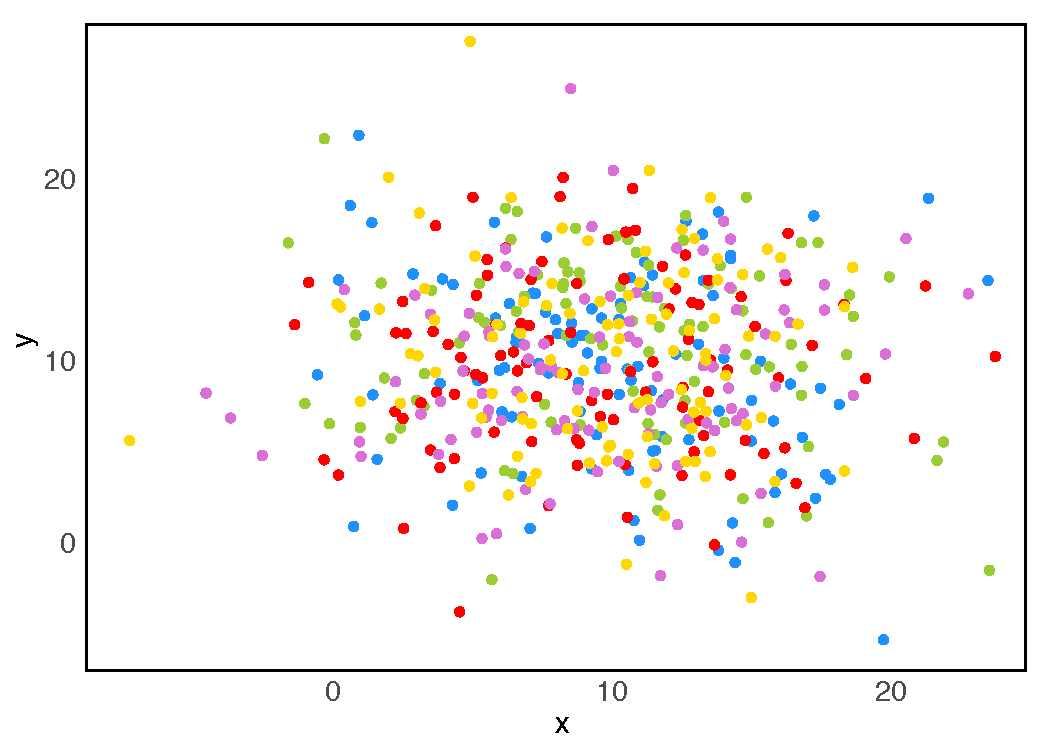
\includegraphics{RandomDotplot_edited.png}
\caption{\textbf{Edited version of the random dotplot, with all black
dots changed to red.}}
\end{figure}

Similarly, if you wanted to change just a spatially defined subgroup of
points (ummm, don't just change points in a graph, as a sidenote), you
can use the lasso tool to accomplish that.

\begin{figure}
\centering
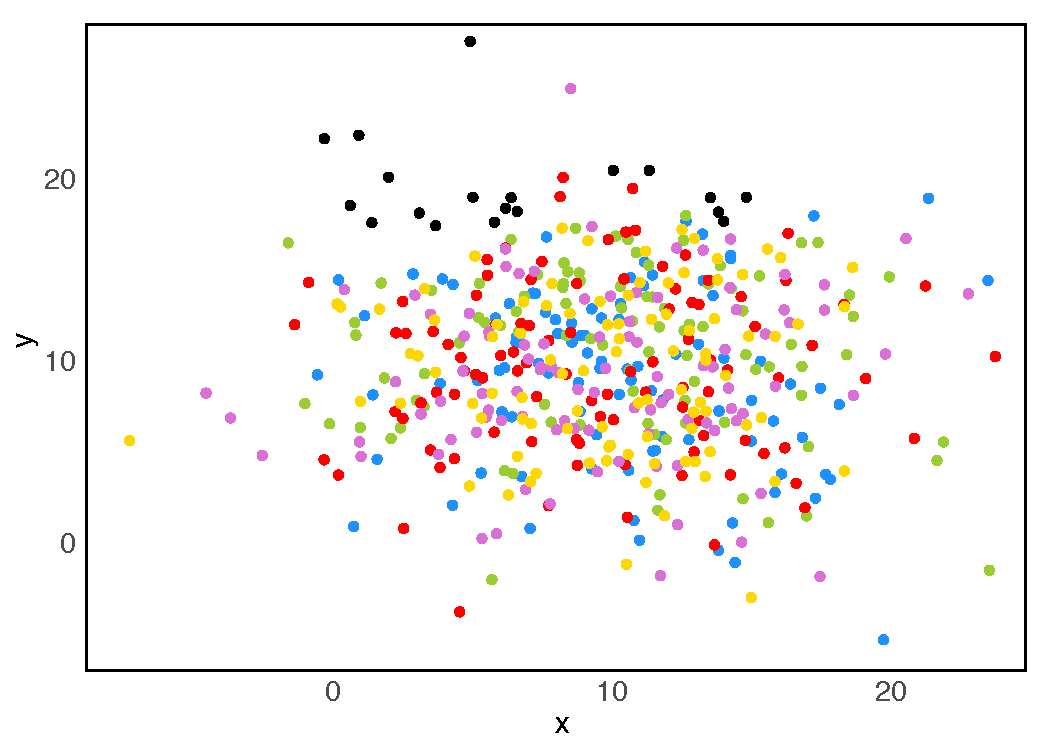
\includegraphics{RandomDotplot_edited2.png}
\caption{\textbf{Edited version of the random dotplot, with a spatially
defined group of dots changed back to black using the lasso tool.}}
\end{figure}

\subsubsection{III. Free anchors and
edges}\label{iii.-free-anchors-and-edges}

\begin{figure}
\centering
\includegraphics{Freeanchors.png}
\caption{\textbf{Drawsies!! The ``Pen'' and ``Curvature'' tools.}}
\end{figure}

The two pen tools are the workhorse tools for anything you're attempting
to draw by hand. This includes all of the silhouettes that you will draw
after this workshop and means that you will have to practice using these
tools quite a bit. I exclusively use the \textbf{Pen Tool} -- I actually
think the \textbf{Curvature Tool} is a feature of newer AI versions, but
it essentially just helps draw pretty curves, which I don't normally
need (or use the ``Arc Tool'' for). In essence, with every click, you
set an anchor point on your canvas. Wherever you move your mouse next,
you will now (as of the 2015 CC version) see an edge that is
automatically calculated. If you click again, said edge actually
solidifies, but you can still shape it my keeping the mouse-click alive
and moving the handles around. This may sound abstract, but will be
fairly intuitive. A few notes about these drawings:

\begin{itemize}
\tightlist
\item
  The pen tool automatically creates lines that you can color, but you
  will only be able to fill drawings that are closed, i.e.~where your
  anchor point of origin is also your final anchor point
\item
  By default, it has both the fill (fill color) and stroke (line color)
  selected. I will get to this shortly, but for now just hit the white
  square with the red diagonal line on the bottom left (see below)
\item
  You can stop-and-go by simply clicking the last anchor you set
\item
  The handles affect both the previous and the next edge by distorting
  it accordingly. If you don't want the distortion to affect your nect
  edge, simply clikc the last anchorpoint to nix the handle.
\item
  try not to make funky loops
\end{itemize}

\begin{figure}
\centering
\includegraphics{fillstroke1.png}
\caption{\textbf{Fill and stroke. More later.}}
\end{figure}

Another thing you'll see is that the Pen Tool has a little white
triangle on the bottom. That means, there's more to unpack! Yay, it's
like Christmas. If you click and hold the pen tool, this little menu
appears:

(Note: if you're ever missing a certain tool, chances are you used a
tool that's usually hidden inside the toolbox and it has temporarily
replaced the main symbol.)

\begin{figure}
\centering
\includegraphics{PenTool2.png}
\caption{\textbf{Pen tool options.}}
\end{figure}

As you may have guessed, you can use these tools to add and delete
anchor points, or to make an anchor point ``live'' again. In short, when
you set an anchor point without holding the mouse to create handles, the
anchor loses its handles. You can re-introduce those by clicking the
anchor with the Anchor Point tool.

\subsubsection{IV. Text and lines}\label{iv.-text-and-lines}

\begin{figure}
\centering
\includegraphics{Textlines.png}
\caption{\textbf{Happy texting and lining with the ``Type'' and ``Line
segment'' tools.}}
\end{figure}

The \textbf{Type Tool} and \textbf{Line Segment Tool} don't really go
together as nicely as the previous ones, but are both pretty
straightforward. The text tool allows you to create and modify text on
your illustrations or graphs. It comes with nearly the entire set of
functions that you get from a regular text processing program (colors,
fonts, subscript, superscript, etc), but on the left side of the
symbols, we're only concerned with actually putting words on paper errr
canvas (um.. screen, actually). It does have a bunch of other tools in
the box with it, which mainly allow you to align text in different ways
(i.e.~inside an object, along a path, etc -- see below)

\begin{figure}
\centering
\includegraphics{TypeTool2.png}
\caption{\textbf{The Type tool is pretty versatile in the creation of
text, but all modification is done elsewhere}}
\end{figure}

The \textbf{Line Segment Tool}, in turn, does excatly what one would
think it does. It makes straight lines using two anchor points and an
edge in between. It also has some reincarnations, like the \textbf{Arc
Tool}, which makes nice little curves, the \textbf{Spiral Tool}, which
is particularly popular among malacologists, the \textbf{Rectangular
Grid Tool} and the \textbf{Polar Grid Tool}.

\begin{figure}
\centering
\includegraphics{LinesBox.png}
\caption{\textbf{Plenty of options in the Line Segment Toolbox}}
\end{figure}

\subsubsection{V. Squares, circles, stars and
more}\label{v.-squares-circles-stars-and-more}

\begin{figure}
\centering
\includegraphics{Squaretool.png}
\caption{\textbf{Making all sorts of shapes with the Rectangle Tool and
toolbox}}
\end{figure}

The \textbf{Square Tool} is a bit of a misnomer, really, since it
harbors a panoply of different shapes. Very similar to all the other
tools, it creates thes shapes by setting geometrically fixed anchor
points and then, by default, fills the area in between the edges. You
can drag these shapes to the preferred size or enter a pre-defined size
on the first click. We're going to disregard the tool on the right, and
instead take a look at all the other shapes we can make. This includes
rounded rectangles (\textbf{Rounded Rectangle Tool}), circles and
ellipses (\textbf{Ellipse Tool}), polygons with the number of corners to
be defined (\textbf{Polygon Tool}), stars with the number of corners (?)
and their radius specified (\textbf{Star Tool}), and, last but not
least, the single least useful tool in the entire GUI: the \textbf{Flare
Tool}, for when you have to make a really weird spacey kind of universe
thing\ldots{} go figure\ldots{}

\begin{figure}
\centering
\includegraphics{Shapes.png}
\caption{\textbf{Oh the possibilities\ldots{}}}
\end{figure}


\end{document}
